%==========================================================================
%>
%>			  This is the main .tex for the 
%>				FUNCTIONAL SPECIFICATION
%>					of PSE Group 10
%>
%=========================================================================%
\documentclass[a4paper]{scrartcl}

% Character encoding
\usepackage[utf8]{inputenc}
\usepackage{arev}
\usepackage[T1]{fontenc}   % 8-Bit-Codierung der Fonts verwenden
 
% Page size
\usepackage[a4paper,top=19mm,bottom=22mm,bindingoffset=10mm,left=10mm, right=15mm,heightrounded,headsep=15mm,includeheadfoot]{geometry} 

% Color for texts and others
\usepackage{color}
\usepackage[usenames,dvipsnames, table]{xcolor}
\usepackage{etoolbox} 
  
% Customized header & footer
\usepackage{fancyhdr}
\pagestyle{fancy}
 \fancyhf{} 	% clears all
	\fancyhead[L]{PSE Group 10 \\ Functional Specification}		% header
	\fancyhead[R]{\leftmark} 
	\renewcommand{\headrulewidth}{0.5pt}
	\rhead{\nouppercase{\leftmark}}
	\patchcmd{\headrule}{\hrule}{\color{Bittersweet}\hrule}{}{}
	
	\renewcommand{\footrulewidth}{0.5pt}						% footer
	\patchcmd{\footrule}{\hrule}{\color{Bittersweet}\hrule}{}{}
	\fancyfoot[C]{\thepage}
	
% Customized headlines
\usepackage{titlesec}
 
 
% If you want enumartions to go on with last one -> do this:
% \begin{enumerate}[resume]
\usepackage{enumitem}
\setlist{leftmargin=*}



%\setlist[1]{labelindent=\parindent}

% Including pictures
\usepackage{graphicx}

% Referring to tables
\usepackage{array}

% Return after CR set 0
\setlength{\parindent}{0pt} 
\setlength{\parskip}{6pt}	% space after passage



% For links of the chapters and out of the pdf + boxes around links deleted
\usepackage[colorlinks=true, linkcolor=black, urlcolor=blue]{hyperref} 


% Glossary 
% \usepackage{ifthen}
% \usepackage{xkeyval}
% \usepackage{xfor}
% \usepackage{amsgen}
% \usepackage{etoolbox} 

\usepackage[makeindex]{glossaries}
\newglossaryentry{SkyServer}
{
  name=SkyServer,
  description={is a big database for astronomical data. It contains pictures
              and other information concerning astronomy and tries to 'form a 
              map of the universe
              }
}


\newglossaryentry{KIT}
{
  name=KIT,
  description={is a technological university in Karlsruhe, Baden-Württemberg, Germany 
              (Karlsruhe Institute of Technology)}
}

\newglossaryentry{log file}
{
  name=log file,
  description={is a file where a large amount of data is saved in one or another form.}
}

\newglossaryentry{.csv}
{
  name=.csv,
  description={is a file-ending which is used for log files, 
  which saves them in a standardized formatting schema.}
}

%Feel free to censor, or whatever
\newglossaryentry{browser}
{
  name=browser,
  description={A piece of software mostly used to navigate the enchanting world of the internet, and thus most commonly
used to watch illegal movies and creep your neighbours photos on facebook. Can be also used to view nice charts.}
}

\newglossaryentry{Firefox}
{
  name=firefox,
  description={A browser that is both modern and popular. Other browsers are popular too, but not modern. }
}

\newglossaryentry{Chrome}
{
  name=chrome,
  description={is a modern browser like firefox, with the notably difference being that google knows about your
creeping of your neighbour. See browser.}
}


   
\makeglossaries   
 

%\author{Lukas Ehnle, 
%Jo Klawitter, Nikos Moraitakis, Alexander Noe, Anas Saber}

%!!!!!!!!!!!!!!!!!!!!!!!!!!!!!!!!!!!!!!!!!!!!!!!!!!!!!!!!!!!!!!!!!!!!!!!!!!!%
\begin{document} % BEGIN BEGIN BEGIN BEGIN BEGIN BEGIN BEGIN BEGIN BEGIN
%!!!!!!!!!!!!!!!!!!!!!!!!!!!!!!!!!!!!!!!!!!!!!!!!!!!!!!!!!!!!!!!!!!!!!!!!!!!%

% Including the customized title page
\newgeometry{a4paper,top=19mm,bottom=10mm,left=15mm, right=15mm, heightrounded,headsep=15mm, includeheadfoot}
\begin{titlepage}

\vspace*{-3cm}
\begin{center}

\begin{tabular}{m{5.5cm} m{5cm} m{5.5cm}}
\arrayrulecolor{Bittersweet!90}

\begin{center}
\footnotesize{
\textbf{ Lehrstuhl für Systeme und Informationsverwaltung}
\newline

Prof.Dr.Ing. Klemens Böhm

Hoang Vu Nguyen

Marco Neumann
} 	
\end{center}
   & 
\begin{center}

   
\includegraphics[width=0.9\linewidth]{Pictures/KIT-Logo.png}
   
\end{center}    
   & 
\begin{center}
\footnotesize{
\textbf{Praxis der Softwareentwicklung (PSE)}\newline
WS 2012/2013\newline

Visualizing and Statistically Analyzing Access Behavior to Scientific Databases
}
\end{center}\\
\hline
 
\end{tabular}


\vspace*{4.6cm}

\Huge
QA \& Testing

\vspace*{1.5cm}

\normalsize

\begin{center}

   
\includegraphics[width=0.7\linewidth]{Pictures/WHAT-LogoText2.png}
   
\end{center} 


\vspace*{2.7cm}

{\color{Bittersweet}\hrule}
\vspace*{0.4cm}
 {\today}
 
\vspace*{0.4cm}
\normalsize

 

\begin{tabular}{r l}

\arrayrulecolor{Bittersweet!90}
\hline
& \\
 
  	Functional Specification
&
	\textbf{Alexander Noe}
\\ 
	Design
& 
	\textbf{Jonathan Klawitter}
\\ 
	Implementation 
& 
	\textbf{Anas Saber}
\\
	QA / Testing 
&
	\textbf{Nikolaos Alexandros Kurt Moraitakis}
\\
	Final 
&	\textbf{Lukas Ehnle}\\

 
\end{tabular}

E-M@il: \href{mailto:pse10-group14-ws12@ira.uni-karlsruhe.de}{pse10-group14-ws12@ira.uni-karlsruhe.de}
% Bottom of the page

\end{center}
\end{titlepage} 
\restoregeometry
\newpage 

\section*{About this document}

\subsection*{General Information}
%\subsection*{Why this specification is written}
\gls{PSE} is a mandatory course for students of computer science bachelor at the % Glossary: PSE, KIT
Karlsruhe Institute of Technology (\gls{KIT}). Therefor groups of five to six
students are formed to write programs of 'medium size'. 
The task given in this course consists of analyzing and visualizing the server log of a \gls{database}.

This specification is the one of \gls{PSE} Group \#10 in the winter semester 2012/13.


%\subsection*{Content of this specification}
\subsection*{What this specification does}
The purpose of this document is an outline of the functional specifications and requirements
for the WHAT application. It tries to give a complete and exact model of the future system.
In the course of this it wants to give the developers answers to all possible question concerning
what should be implemented.


\subsection*{What this specification does not}
This specification does not give any information on how the system should be implemented. 
Also it doesn't contain any project planning or deadlines.


\subsection*{A 'Living Document'}
Software development is a dynamic process. So with proceeding development the
content of this specification will change continuously. 


\subsection*{Skyserver}
The concept of the system described in this specification should work with any \gls{database}
storing it's query-log. The \gls{SkyServer} will function
as an example and testing reference for this system. 
\gls{SkyServer} is one of the biggest \glspl{database} for astronomical data.
 
% \subsection*{About us}
% %\subsection*{About the writers}
% Because no one of us speaks English as his first language,
% we can't guarantee that our documentation doesn't contain simple
% or incorrectly used language. Our focus lies more on
% having an easy-to-understand and correct documentation
% than on perfect English.% by a native speaker.

\subsection*{Questions and comments}
If you have any questions or comments regarding this document feel free to send us an 
 \href{mailto:pse10-group14-ws12@ira.uni-karlsruhe.de}{E-Mail} at 
 \href{mailto:pse10-group14-ws12@ira.uni-karlsruhe.de}{pse10-group14-ws12@ira.uni-karlsruhe.de}.







 
% \newpage
% \section*{Introduction} % obsolet?
% PSE is a mandatory course for students of Bachelor Informatik in the
% Karlsruhe Institute of Technology (KIT).
% In this course we have to form groups of five or six people to write
%  a program of 'medium size' ($\sim$5000 Lines of Code).
% 
% Our task given in this course consists of
% analyzing and visualizing the server log of the
% \href{http://skyserver.sdss.org/public/en/}{SkyServer}.
% This is one of the biggest public databases for astronomical data.
% It contains pictures and informations of astronomical data
% and tries to form a 'map of the universe'.
% 
% This assignment is one of two assignments which will be handled
% in English.
% Because no one of us speaks English as his first language,
% we want to apologize that our documentation may contain simple
% or in some parts incorrectly used language. Our focus lies more on
% having easy-to-understand and correct documentation
% than on perfect English, which looks like written by a native speaker.
% 
% We are going to write a web-frontend in javascript allowing users
% to access the finished application from everywhere
% with recent browsers. The actual application can be spliited into two
% different parts. The first part - which will be referred as 'Parser' and is going to convert the CSV-formatted
% serverlog from Skyserver into a data-warehouse. It will
% be accessible via admin-login to the webpage where we can enter a
% logfile, which will be parsed into our warehouse.
% The second part - which will be referred as 'Analyzer' works on this data-warehouse
% and allows every user of our webpage to create various charts,
% for example scatterplots and histograms.
% Due to the fact that we split our project in two smaller parts,
% many parts of this specification are going to be splitted in two.
% 
% We have to state that no one of us has much experience in working
% with databases and javascript.
% Therefore we can't guarantee the correctness of all information
% stated in this specification. Some of the specifications may be altered when we design or
% implement the actual program.
 
\tableofcontents
  
\newpage 
\section{Goals}

%=======================================================================

%Through or with?
With this program the user should be put in the position 
to visualize the prepared data of queries, made against his data base.


To structure the criteria the system has to fulfill, 
it is divided into three parts for this and other sections.
\begin{itemize}
  \item Web page
  \item Parser
  \item Analyzer
\end{itemize}
See \ref{overview} for an overview of these parts and their relationships.
In the following section their specific goals and criteria are described.
 

% \subsection{Core criteria}
% This criteria have to be fulfilled to guarantee 
% the core functionality of the system.
% 
% \begin{itemize}
%   \item Provide an option to import CSV-formatted log files % glossary
%    and parse specified data out of them
%   \item Load 
% \end{itemize}


%=======================================================================
\subsection{Web page}
\subsubsection{Core criteria}
\begin{itemize}
\item The web page is the graphical interface for users and administrators. 

\item Users can choose the charts they want to see 
and also choose and filter the dimensions and measures for those. 
It has to support at least scatter plots, histograms and bubble charts.

\item The web page provides help for how to use the diagrams and variables (dimensions 
and measures). 
Also the navigation on the page is easy to use and straight forward.

\item An admin-login provides administrative rights, which are needed to use the parser.
\end{itemize}

%----------------------------------------------------------------------
\subsubsection{Optional criteria}
\begin{itemize}
\item The language of the website can be changed (e.g. German).

\item The administrator gets the ability to handle the data warehouse and load new log-files.

\item A little history of the last requested charts is stored and viewable.
\end{itemize}

%----------------------------------------------------------------------
\subsubsection{Exclusion criteria}
\begin{itemize}
\item The web page does not allow normal users to load new data into the data warehouse.

\item The web page does not provide statistical tables. 
\end{itemize}


%=======================================================================
\subsection{Parser}

\subsubsection{Core criteria} % Musskriterien
\begin{itemize}
\item The Parser is able to perform the ETL-process on CSV-formatted log files (from Skyserver). %glossary
This means it extracts the data it needs from the files, transforms them 
and loads them into the data-warehouse. Dimensions and measures are specified in \ref{WHschema}.
  
\item The Parser will recognize invalid logs and won't add them to the data-warehouse.
 Every log with a mistake won't be accepted, because an error-message is not 
 as bad as a corrupted data-warehouse. 
 
\item The Parser will be fed with log files from the administrator via web page.
\end{itemize} 

% %----------------------------------------------------------------------
% \subsubsection{Optional criteria}
% \begin{itemize}
% \item 
% \end{itemize} 
 
%----------------------------------------------------------------------
\subsubsection{Exclusion criteria}
\begin{itemize}
\item This parser is only able to operate on CSV-formatted logs from SkyServer. 
It can neither read logs in another formats nor logs from another source.

\item There is no way to avoid using this Parser when adding data to the warehouse. 
This can stop corrupting the warehouse to guarantee correct data in the warehouse.

\item The Parser doesn't correct mistakes in the log file.
\end{itemize}



%=======================================================================
\subsection{Analyzer}

\subsubsection{Core criteria}
\begin{itemize}
\item The analyzer is the gate to the data warehouse. It extracts the specific data, 
needed for the diagrams, passing them to the java-script front-end.
\item The analyzer can take filtered information via web page from the user 
to use only certain data for the charts.
\item The charts that are supported are at least:
\begin{itemize}
\item scatter plots
\item histograms
\item bubble charts
\end{itemize}

\end{itemize}

%----------------------------------------------------------------------
\subsubsection{Optional criteria}
\begin{itemize}
\item The analyzer will support more chart-types, for example the combination of
a histogram and a scatter plot. 
\item The analyzer does a little bit of data mining, and presents some potentially interesting information.
\end{itemize}

%----------------------------------------------------------------------
% \subsubsection{Exclusion criteria}
% \begin{itemize}
% \item 
% \end{itemize}


% Vll sollte man noch was zum warehouse sagen.




\newpage 
\section{Usage}
%Relevant
% http://www.geekherocomic.com/comics/2009-02-06-prima-donna-developer.png
\subsection{Applications}
Let's say you have some data in a database(who hasn't, right?).
Let's say you don't feel like wasting your only life and what to see what parts of that data ara important, fast.
Let's say you don't have the time, incination, or even (gasp!) technical background to do so yourself.

Fear not. WHAT is exactly what you are looking for, and more!
With features such as drawing of scatterplots, histograms, bubble charts* 
and other obscure charts you have never heard of before, statistics about the importance of your tables*,
automatic reports of* of interesting correlations*, what is the right tool for your job!

As a concrete implementation, all this will be provided for the SKYSERVER logs dataset, but other datasets may be
used as well, with minor or not as minor modifications.

(* indicates that this is not a core feature, may be included later in the project, or not at all.)

\subsection{Target groups / Audience}

The target group of this application are people that want to analyze 
and visualize the amount of queries runned against their database -or like
in our case - against the SkyServer.

No matter if operating on a private or a public database, this implies
\begin{itemize}
  \item the people that run the database wanting to optimize the access to
  	their data,
  	
  \item people that are interested from where the database is used,

  \item people knowing or using the database, wondering for what and when other people
  use the database,
  
  \item people new to the database, wanting to know, what may be of interest
  on the database.

\end{itemize}
To summarize briefly, WHAT will be of interest for many people, 
whether running the database, making market research or just all the folks
loving statistics and diagrams.

% \begin{enumerate}  
%   \item people that know about the skyserver. Since the skyserver only 
%    allows queries via sql and has an arcane website this greatly 
%    reduces the prospective audience. We do not expect the webserver 
%    to run into scaling issues.
%   
%   \item People that are interested in what other people are 
%   using the web server for. Our project mainly visualizes sql queries
%    from other people. Knowing sql, while not a prerequisite, 
%    would allow the user to fully utilize the software.
%   
% \end{enumerate}


We exspect a audience knowing by themself what they want to know. This means,
there should not be real suppourt chosing useful variables and scales for
the charts. 

Also we exspect adminstrators to be well versed with technical matters.

% This is a technical audience.
% 
% That said, this does not prevent the (web) user interface from being functional,
%  usable and prettier than what you would expect a group of 
%  computer science students to design.
 

\subsection{Operating conditions}

The program is mainly used as a website, with the primary difference being
 that the server has to be started if the capacity for it to run 
 all the time on a dedicated machine doesn't exist. 
 %this is formal english for: we do not have a server. Gibe server plos
The program needs a server to run. 

If a dedicated server exists, the program can be used from anywhere
 with a decent network connection with the server.

If not, the program can still be run on the same computer as 
the server (on localhost), but the server will have to be started first.
 


\newpage 
\section{Operating environment}



%You keep using that word. I don't think it means what you think it means
% http://en.wikipedia.org/wiki/Workstation
Whereas the programm and the data warehouse run on a sever,
the access to it will be via a web browser on the users computer. 
This implies that the webpage will need to be hosted on a webserver.



\subsection{Software}
\begin{itemize}
  \item The server hosting the data warehouse needs  MySQL %glossary
  
  \item The server hosting the web page needs a 
  recent version of th Java Runtime Environment / Java VM  % Glossary
\end{itemize}


This software is required on the users computer:
\begin{itemize}
  \item Latest version of a modern browser
  \begin{itemize}
    \item Chrome and Firefox will be supported
  \end{itemize}
  \item JavaScript (enabled)
\end{itemize}



\subsection{Hardware}

The server has to be fast enough to support all clients. This depends on
the expected number of clients. Most computations will be done on the server.

% Is the program really local hosted? 
The client needs to be fast enough to visualize the data received from the server, as that's almost all it does.
The required hardware thus depends greatly on the amount of data that needs to be 
visualized. That said, any recent computer, with for example, 
an Intel® Core™2 Duo CPU E8400 @ 3.00GHz × 2 processor, 
4GB(2x2GB) of 667Mhz DDR2 SDRAM, running Ubuntu Linux 12.10 Quantal Quetzal, 
% this was, like, a joke, because it's, like, my computer
as a point of reference, should be able to visualize about 50.000 
data points on a scatterplot with ease.


\subsection{Orgware}

The server needs to be able to connect to the client with a reasonable latency.
Also it has to be set up before the client will be able to connect to it.

% Other direction: Program hast to be able to run query against data warehouse?

To fulfill optional requirements, the program musst be able to run queries against
the origin database. 

\subsection{Product interfaces}

To fulfill optional requirements .csv files have to be imported.
\newpage
\setlist{leftmargin=40pt}
\section{Functional requirements}


%\renewcommand{\theenumi}{/F\ifnum\value{enumi}<10 0\fi\arabic{enumi}0/}
\renewcommand{\theenumi}{/F\arabic{enumi}0/}
\renewcommand{\labelenumi}{\theenumi}

  
\subsection{Main functions}

This functions are required to fulfill the core criteria.
 
\subsubsection*{General}
\begin{enumerate}
  \item Provide access via web page\label{f1}
    
  \item Provide option for chart types\label{f2}
  
  \item Show diagrams\label{f3}
  
  \item Show histograms\label{f4} % add to glossary
  
  \item Provide option for the two variables of the histogram\label{f5}
  
  \item Provide option for the interval 
  or selection of the x-axis variable\label{f6} % ref to privious
  
  \item Show scattered plots\label{f7} % add to glossary
  
  \item Provide option for the 
  two variables of the scattered plot\label{f8}
  
  \item Provide option for the intervals 
  or selections of the two variables\label{f9} % ref to privious
  
  \item Show bubble charts\label{f10} % add to glossary
  
  \item Provide option for the three variables
   of the scattered plot\label{f11}
  
  \item Provide option for the intervals 
  or selections of the three variables\label{f12} % ref to privious
  
  \item Show information about chart types\label{f13}
  
  \item Show information about selectable variables\label{f14}
  
\end{enumerate}


\subsubsection*{Administrator specific}
This functions are required for the administrative business.

\begin{enumerate}[resume]
  
  \item Provide access via web page with administrator rights\label{f15}
   
  \item Provide the opportunity to pass log-files to the parser\label{f16}
   
\end{enumerate}


\subsubsection*{Parser specific}
 
 The following functions specify the parses functionality.
 Thereby \ref{p2} to \ref{p4} specify the function \ref{p1}.
 
\begin{enumerate}[resume]
  
  \item Extract specific data from the log-files \label{p1}
  
  \item Extract access database, access time and user information (dimensions)\label{p2} % add to glossary: first
  
  \item Extract number of rows, elapsed time, busy time (measures)\label{f17} % add to glossary: all 3
  
  \item Extract type of data requested from the \texttt{where}-part\label{p4} % add to glossary: where
  
  \item Transform the data to fit into the data warehouse schema\label{f18}
  
  \item Load the data into the data warehouse\label{f19}

\end{enumerate}

\subsubsection*{Analyzer specific}
 
\begin{enumerate}[resume]
  
  \item Run specific queries against data warehouse \label{f20}
  
  \item Transform received data serving the web page \label{f21}

\end{enumerate}


\subsection{Extending functions}

To fulfill the optional goals the following functions are required.

\subsubsection*{General}
\begin{enumerate}[resume]
  
  \item Select language on web page \label{f22}
  
  \item Show bubble map \label{f23} % add to glossary
  
  \item Show combination of histogram and scattered plot \label{f24}
  
  \item Show other diagrams and charts \label{f25}
  
  \item Show history of the 5 last requested charts \label{f26}
  %Niko's Data Mining follows
  %
  % Where clusters are probably observed
  \item Show interesting attribute combinations

  % But visualize them. In different colors and stuff
  \item Show clusters in the data
  %We don't want the server to be too slow. Clustering requires cpu time
  
  \item Add background clustering
  
  \item Turn background clustering on and off //to make the program faster


 
\end{enumerate}


\subsubsection*{Administrator specific}

\begin{enumerate}[resume]
   
  \item Provide the opportunity to initialize the data warehouse\label{f27}
   
  \item Provide the opportunity to request new log-files for specific time intervals
  	from the database \label{f28}
  
  \item Provide the opportunity to clean the data warehouse \label{f29}
   
\end{enumerate}



\newpage 
\section{Data}
The product data are divided in two groups, static data, 
which are delivered with the program and in 

% Enumeration changed
\renewcommand{\theenumi}{/D\arabic{enumi}0/}
\renewcommand{\labelenumi}{\theenumi}

\subsection{Static Data}

\begin{enumerate}
  \item Language files
  \item Manual
  \item Source Code
  \item Documentation
  \item Graphics for GUI
  \item HTML backbone
  \item Javascript files
  \item Stylesheet files
\end{enumerate}

\subsection{Dynamic Data}


\subsection{Data-Warehouse data} 

The warehouse may use a star schema. It will store nearly all d

The data warehouse stores all the data, coming from from the database (Skyserver) server logs.
They were subject of the ETL-process in the parser. If optional criteria are fulfilled
 they can be replaced by clearing the data warehouse 
 and loading new data via web page as administrator.

The data warehouse may use a star schema.
\begin{center}
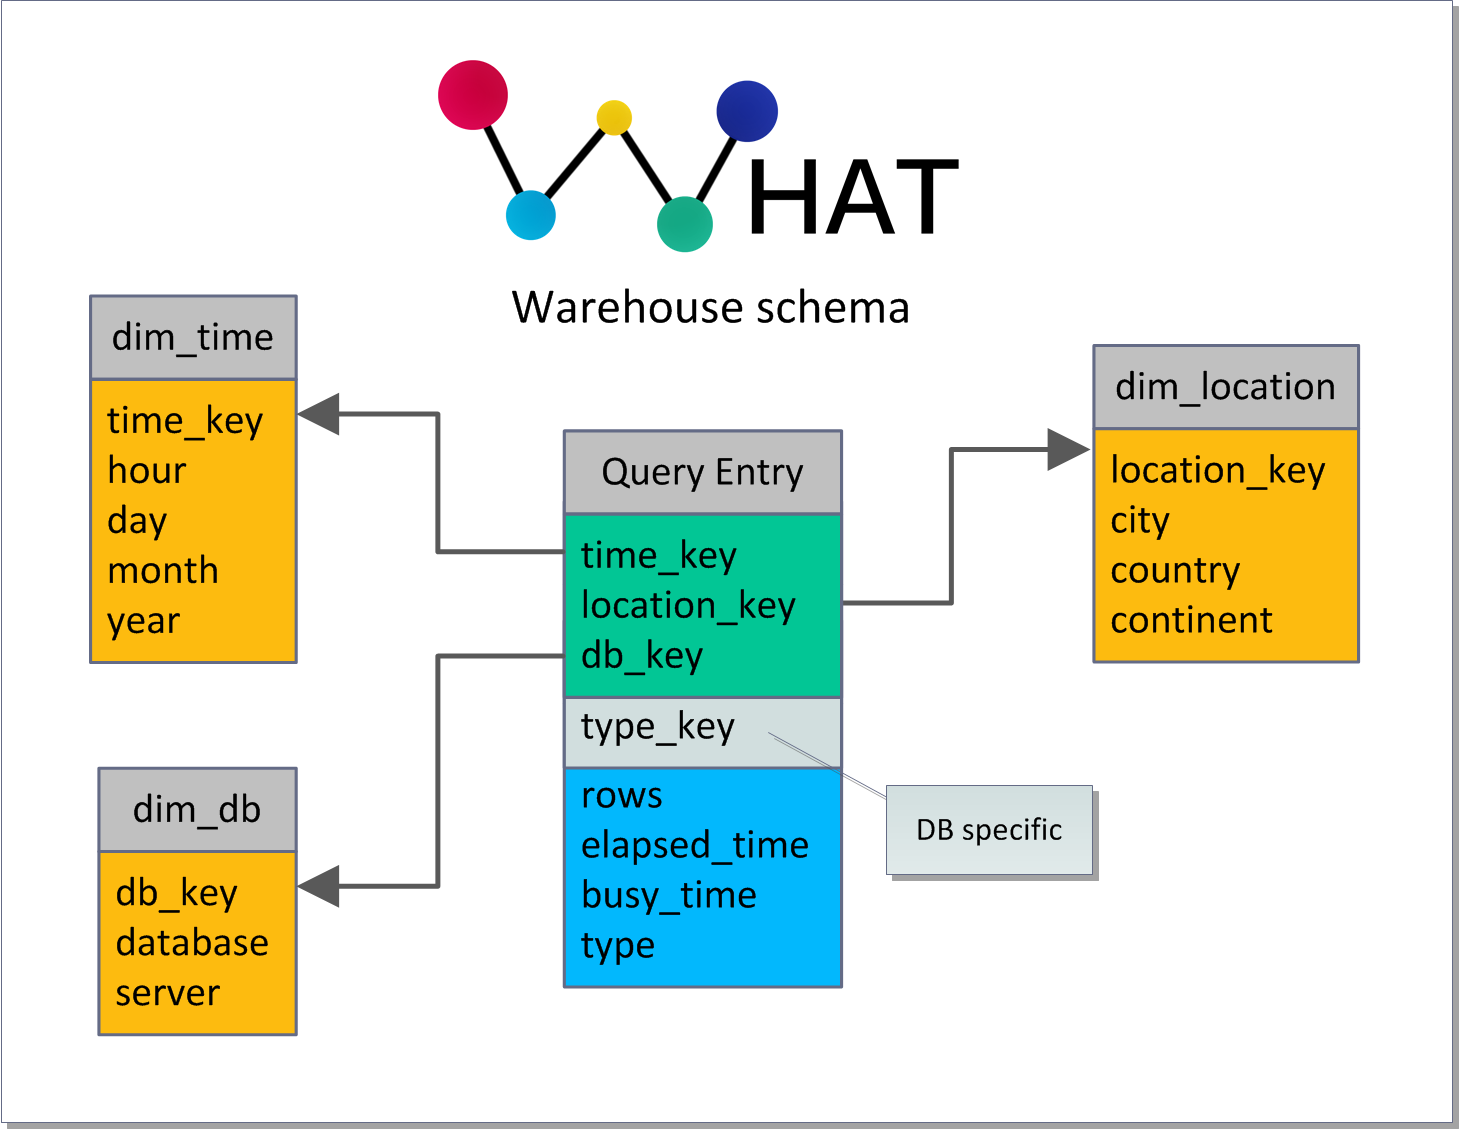
\includegraphics[width=0.7\linewidth]{Pictures/WareHouseSchema.png}
\end{center}   
See rows, elapse time and bussy time in the glossary (\ref{glos}) for descriptions. 


% \begin{enumerate}[resume] % <- resume goes on with old counter
%   \item Database accessed by Users
%   \item Server accessed by Users
%   \item City of Users
%   \item Country of Users
%   \item Time of SkyServer access
%   \item Number of rows accessed
%   \item Elapsed time of access
%   \item CPU busy time of access
% \end{enumerate}

% we may include just the schema in here? 
\newpage 
\section{Nonfunctional requirements}
\newpage 
\section{Test Cases}


% Enumeration changed
\renewcommand{\theenumi}{/T\arabic{enumi}0/}
\renewcommand{\labelenumi}{\theenumi}

\subsection{General}

Those test-cases are necessary for the webpage to work 
properly and succeed in serving basic requests.

\begin{enumerate}

\item Access web page (\ref{f1})
\begin{enumerate}
  \item[/T12/] via Google Chrome,
  \item[/T14/] via Mozilla Firefox.
\end{enumerate}
\label{t10}

\item Navigate switfly through the web page. (\ref{f141}) 
\label{t11}

\item Open page for scatter plot-creation and create an example
      with x-Axis date and y-Axis number of lines per request. (\ref{f2}, \ref{f3}, \ref{f7}, \ref{f9})
\label{t12}

\item Open page for histogram-creation and create an example
      with x-Axis year and y-Axis number of requests. (\ref{f2}, \ref{f3}, \ref{f4}, \ref{f6})
\label{t13}

\item Open page for bubble chart-creation and create an example
      with x-Axis year, y-Axis Country and size number of requests. (\ref{f2}, \ref{f3}, \ref{f10}, \ref{f11})
\label{t14}

\item Call the information about chart types. (\ref{f13})
\label{t15}

\item Request information about selectable variables. (\ref{f14})
\label{t16}

\end{enumerate}

\subsection{Administrator specific}

Those test cases check the correct admin-login.

\begin{enumerate}[resume]

\item Enter loginname and password for admin-login. (\ref{f15})
\label{t17}

\item Log-in and get administrative rights. (\ref{f15})
\label{t18}

\item Try to log in with wrong loginname. (\ref{f15})
\label{t19}

\item Try to log in with wrong password. (\ref{f15})
\label{t20}

\item Pass example log-file to the parser. (\ref{f16})
\label{t21}


\end{enumerate}

\newpage
\subsection{Parser specific}

The following test cases test the correct work of our parser.
%, which extracts information from a .csv-file and writes 
%it in our data-warehouse.

\begin{enumerate}[resume]

\item Parse example log-file and extract valuable information correctly. (\ref{p1})
	\\ More specifically: 
\label{t22}
  \begin{enumerate}

	\item[/T132/] Extract correct database, time, user information 
	and type, (\ref{p2})
\label{t23}

	\item[/T134/] Extract correct number of rows, elapsed time, 
	busy time from the log-file, (\ref{f17})
\label{t24}	
	
	\item[/T136/] Extract the type requested. (\ref{p4})
\label{t25}

  \end{enumerate}

\item Load extracted information into the data warehouse correctly. (\ref{f18}, \ref{f19})
\label{t26}

\end{enumerate}


\subsection{Analyzer specific}

The functions  \ref{f20} and \ref{f21} of the analyzer are 
already tested in the general test-cases \ref{t12} to \ref{t14}.



% \subsection{Scenario Testing}
% 
% Scenario testing is sequence Workflow from use cases and shod lead iteratively
% 
% % % Enumeration changed
% % \renewcommand{\theenumi}{/T\arabic{enumi}0/}
% % \renewcommand{\labelenumi}{\theenumi}
% 
% \subsubsection {Scenario 1: loading logs file} 
% 
% \begin{enumerate}
%  
% \item Start the Application
% 
% \item Log in the User with the Admin ID and password
% 
% \item Write the Queries
% 
% \item Send the Querise to Skyserver
% 
% \item Send the logs file to parse
% 
% \item Call the opportunity to initialize the data warehouse
% 
% \item Call the opportunity to request new log-files for specific time intervals from the
% database
% 
% \item Call the opportunity to clean the data warehouse %what's mean?
% 
% \item Leave the Application
% 
% \end{enumerate} 
% 
% \subsubsection {Scenario 2: parsing} 
% 
% \begin{enumerate}
% 
% \item Start the Application
% 
% \item Log in the User with the Admin ID and password
% 
% \item Call Extract specific data from the log-files
% 
% \item Call Extract access database, access time and user information (dimensions)
% 
% \item Call Extract number of rows, elapsed time, busy time (measures)
% 
% \item Call Extract type of data requested from the where-part
% 
% \item Call Transform the data to fit into the data warehouse schema
% 
% \item Load the data into the data warehouse
% 
% \item Leave the Application 
% 
% \end{enumerate} 
% 
% \subsubsection {Scenario 3: selecting variables of diagrams} 
% 
% \begin{enumerate}
% 
% \item Start the Application
% 
% \item Select a diagram type
% 
% \item Show the diagram
% 
% \item Call option for the tow or three variables of the diagram
% 
% \item Change one, tow or three variables of the diagram
% 
% \item Refresh the Information
% 
% \item Show the new diagram with new variables of the diagram
% 
% \item Leave the Application
% 
% \end{enumerate}
% 
% \subsubsection {Scenario 4: options} 
% 
% \begin{enumerate}
% 
% \item Start the Application
% 
% \item Call the option menu
% 
% \item Select the Languge of the Application
% 
% \item Show the Application with the selected languge
% 
% \item Leave the Application
% 
% \item Start the Application 
% 
% \item Select the diagram 
% 
% \item Call file menu
% 
% \item Save the diagram as a PDF file
% 
% \item Leave the Application
% 
% \end{enumerate}
% 
% \subsubsection {Scenario 5: A!} 
% 
% \begin{enumerate}
% 
% \item blabla
% 
% \end{enumerate}

\newpage 
\setlist{leftmargin=*}
\section{Models}

\subsection{User stories}

As a user, want to get some Information from skyserver to analyze the database of this server and want to know, how many 
user or client that used this server from wich Countries and in wich time (Month and Year) . 

To analyze this Information in best way, i would like to get Visualizing and Statistically of these Information.
That's mean, i can get some diagram with axises like histogram.

Steps to descrip how can a normal user use this Application:

\renewcommand{\theenumi}{\arabic{enumi}}
\renewcommand{\labelenumi}{\theenumi}

\begin{enumerate}

\item Start internet browser

\item Vist www.say pse10-analyzer.edu web page

\item 

\end{enumerate}

\subsection{Object models}

\subsection{Dynamic models}

\subsection{Web interfaces}

\newpage
\subsection{Overview}\label{overview}
This picture describes the generell concept of WHAT.
\begin{center}
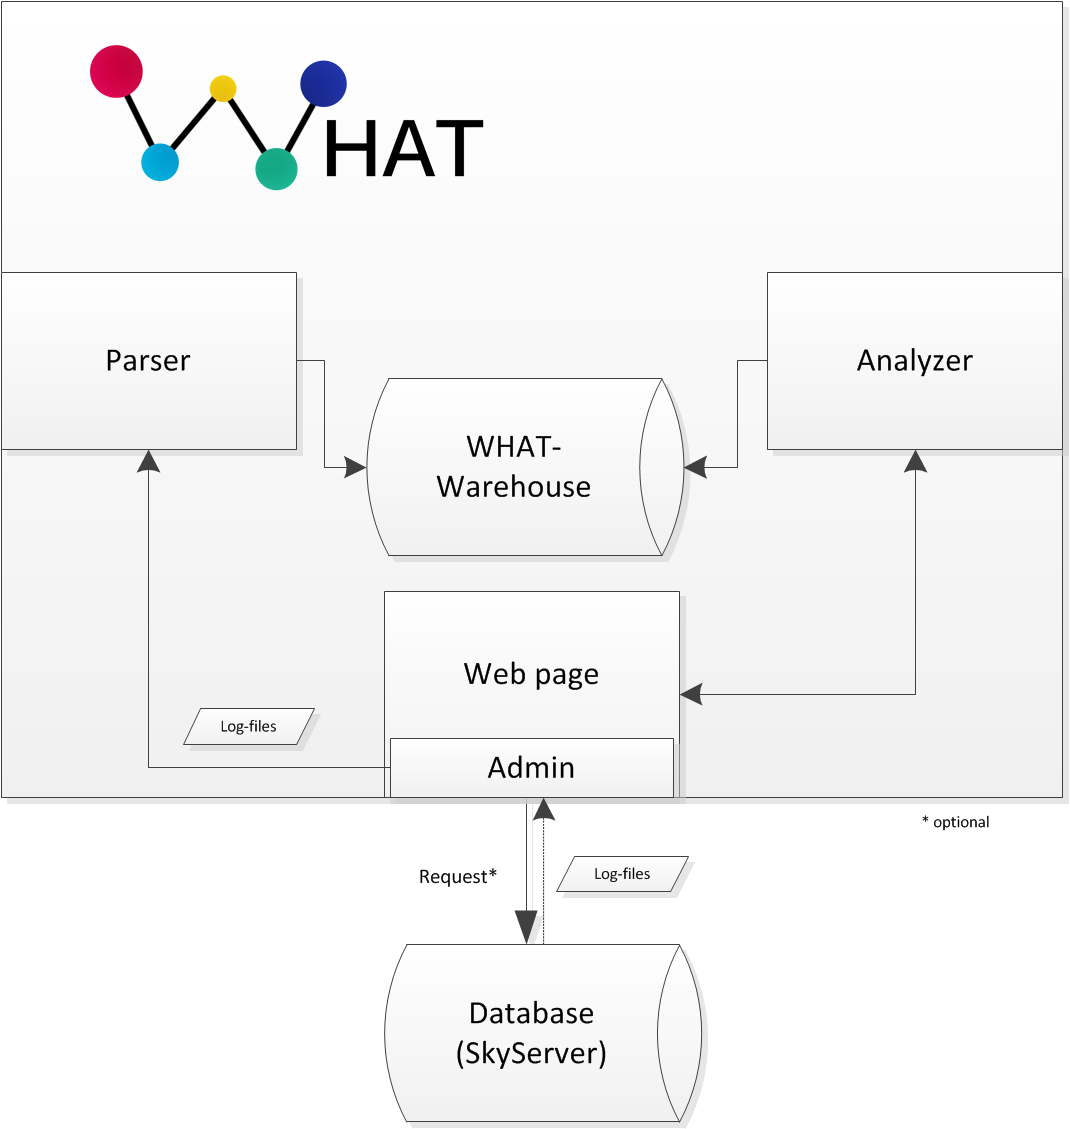
\includegraphics[width=1\linewidth]{Pictures/GenerellConcept.png}
\end{center} 

\subsubsection{Parser}
Parser blabla
\subsubsection{Analyzer}
\subsubsection{Web page}

\subsection{Warehouse schema}\label{WHschema}
The warehouse may use a star schema.
\begin{center}
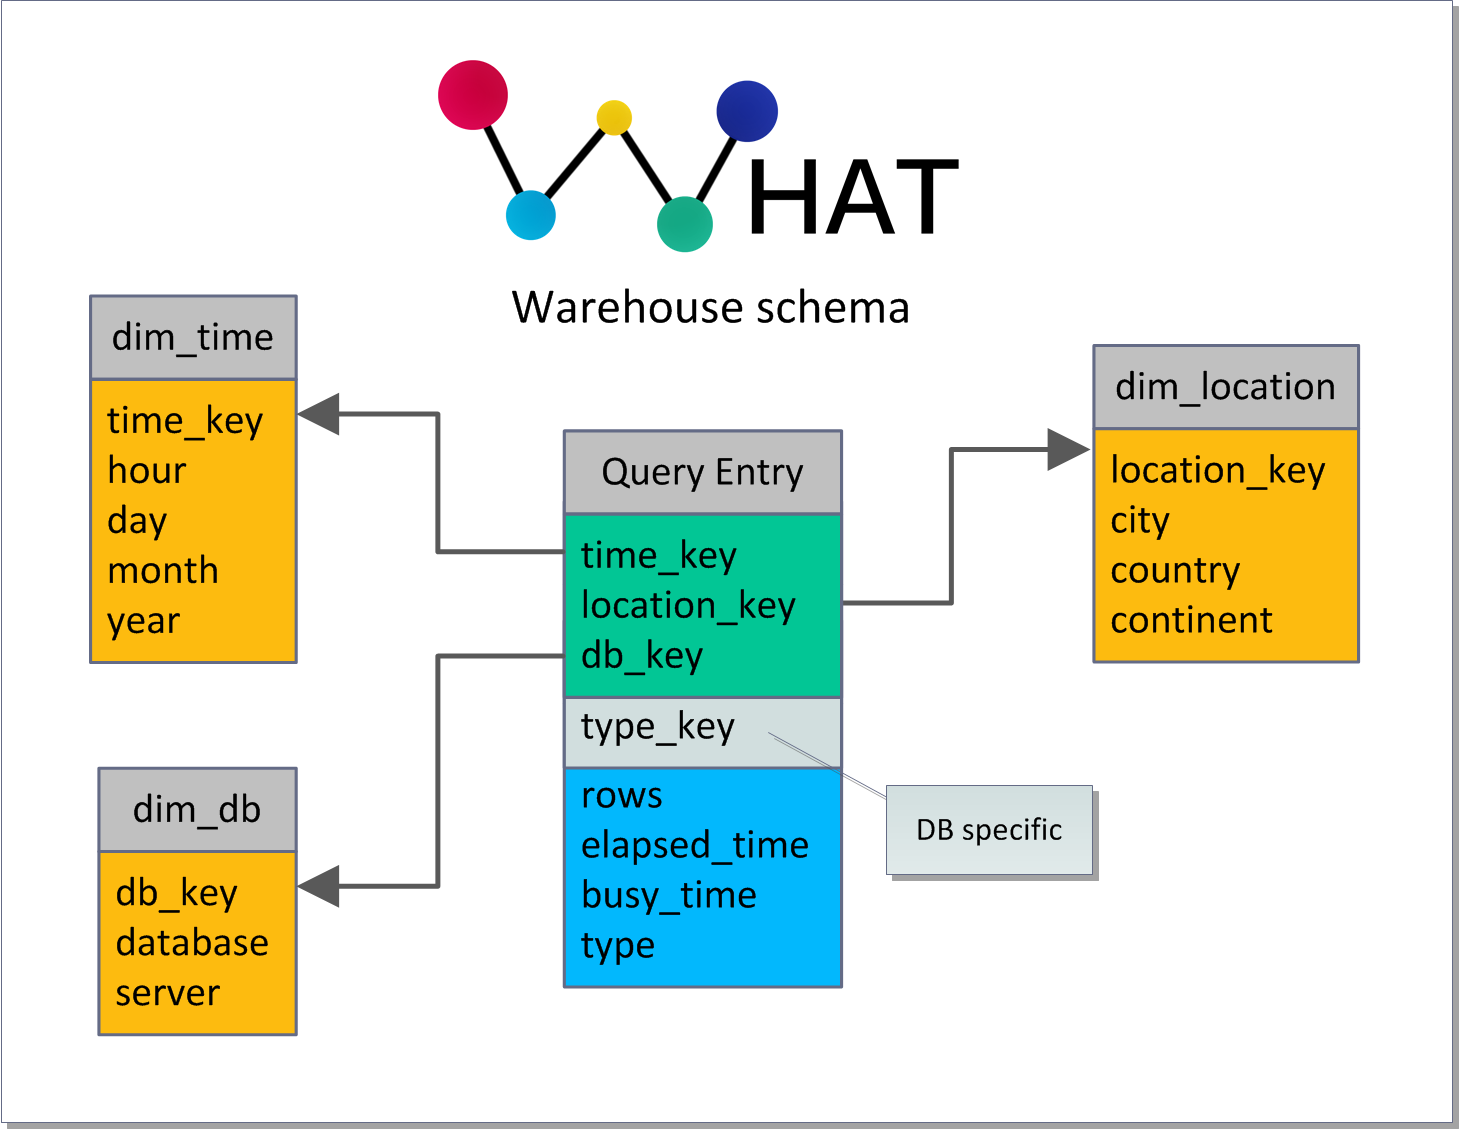
\includegraphics[width=1\linewidth]{Pictures/WareHouseSchema.png}
\end{center}    
\newpage 
\section{Development Environment}

\subsection*{Operating System}
\begin{itemize}
\item Windows 7
\item Fedora 17
\item Whatever Niko uses - EDIT THIS, NIKO!
\end{itemize}
\subsection*{Object Models}
\begin{itemize}
\item Microsoft Visio
\end{itemize}
\subsection*{Version Control}
\begin{itemize}
\item Git
\end{itemize}
\subsection*{Miscellaneous}
\begin{itemize}
\item Github (Hosting of Repository, Issue Tracking)
\item Travis (Integration)
\item {\LaTeX} (Documents)
\item Gradle (Building) 
\end{itemize}
\newpage
\setlist{leftmargin=90pt} 
\section{Glossary}


\newpage 
   
%!!!!!!!!!!!!!!!!!!!!!!!!!!!!!!!!!!!!!!!!!!!!!!!!!!!!!!!!!!!!!!!!!!!!!!!!!!!%
\end{document}  % END END END END END END END END END END END END END END 
%!!!!!!!!!!!!!!!!!!!!!!!!!!!!!!!!!!!!!!!!!!!!!!!!!!!!!!!!!!!!!!!!!!!!!!!!!!!%
